\begin{ex}[Genus $2$ surface]
Let us consider the genus $2$ surface $\Sigma_2$.
Take $S$ to be a separating curve, going once around between the two holes,
as in Figure \ref{fig:genus2}. Consider the Dehn twist $\tau_S$ around $S$.
\begin{figure}[ht]
\centering
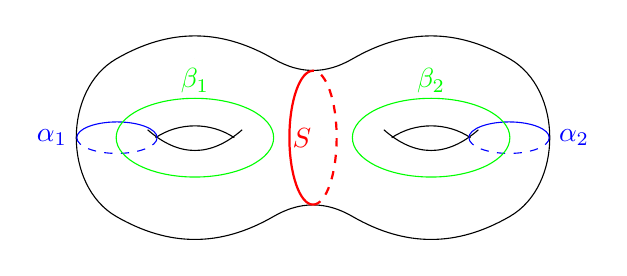
\begin{tikzpicture}
\draw[smooth] (0,1) to[out=30,in=150] (2,1) to[out=-30,in=210] (3,1) to[out=30,in=150] (5,1) to[out=-30,in=30] (5,-1) to[out=210,in=-30] (3,-1) to[out=150,in=30] (2,-1) to[out=210,in=-30] (0,-1) to[out=150,in=-150] (0,1);
\draw[smooth] (0.4,0.1) .. controls (0.8,-0.25) and (1.2,-0.25) .. (1.6,0.1);
\draw[smooth] (0.5,0) .. controls (0.8,0.2) and (1.2,0.2) .. (1.5,0);
\draw[smooth] (3.4,0.1) .. controls (3.8,-0.25) and (4.2,-0.25) .. (4.6,0.1);
\draw[smooth] (3.5,0) .. controls (3.8,0.2) and (4.2,0.2) .. (4.5,0);
\draw[blue] (-0.5,0) arc(180:0:0.51 and 0.2);
\draw[blue, dashed] (-0.5,0) arc(180:0:0.51 and -0.2);
\filldraw[blue] (-0.5,0) circle (0pt) node[anchor=east]{$\alpha_1$};
\draw[red, thick] (2.5,-0.85) arc(270:90:0.3 and 0.85);
\draw[red,dashed,thick] (2.5,-0.85) arc(270:450:0.3 and 0.85);
\filldraw[red] (2.6,0) circle (0pt) node[anchor=east]{$S$};
\draw[blue] (5.5,0) arc(180:0:-0.51 and 0.2);
\draw[blue, dashed] (5.5,0) arc(180:0:-0.51 and -0.2);
\filldraw[blue] (5.5,0) circle (0pt) node[anchor=west]{$\alpha_2$};
\draw[green] (1,0) ellipse (1 and 0.5);
\filldraw[green] (1,1) circle (0pt) node[anchor=north]{$\beta_1$};
\draw[green] (4,0) ellipse (1 and 0.5);
\filldraw[green] (4,1) circle (0pt) node[anchor=north]{$\beta_2$};
\end{tikzpicture}
\captionsetup{justification=centering}
    \caption{Genus $2$ surface with Lagrangian sphere $S$.}
    \label{fig:genus2}
\end{figure}

As in \cite{seidel96} we can work over $\Z_2$ instead of the Novikov field,
and the Floer cohomology groups are $\Z$-graded.

$\tau_S$ splits into the product of two anti-symplectic involutions:
Take $c$ to be the anti-symplectic involution which is a reflection along $S$.
It is straight forward to check that $\tilde{c}:=c \circ \tau_S$ is an anti-symplectic involution.
\begin{comment}
\begin{align*}
(c_+ \circ \tau_S)^ 2 &= 
\begin{cases}
	c_+^ 2  \qquad \text{outside blue region}\\
	(c_+ \circ \tau_S)(q + \nu(p), -p) 
	\qquad \text{inside blue region with coordinates} (q,p).
\end{cases}\\
&=
\begin{cases}
	id \qquad \text{outside blue region}\\
	(q + \nu(p)+\nu(-p), p) = (q,p)
	\qquad \text{inside blue region with coordinates} (q,p).
\end{cases}
\end{align*}
\end{comment}
\noindent In particular, we can write $\tau_S = c \circ \tilde{c}$.

Let us compute $c_*\colon HF^*(\tau^{-1}_S) \to HF^*(\tau^{-1}_S)$.
By the isomorphism (\ref{Iexamples:thm:pedrotti}) Floer cohomology of $\tau^{-1}_S$ is
\begin{align*}
 HF^*(\tau^{-1}_S) &\cong H^*(\Sigma \backslash S; \Z_2)\\
    &\cong  H^*(\Sigma \backslash S;\Z_2) \\
    &\cong H^*(S^1 \vee S^1;\Z_2)
     \oplus H^*(S^1 \vee S^1;\Z_2)\\
     &\cong \Z_2 [pt_1] \oplus \Z_2 \alpha_1 \oplus \Z_2 \beta_1
     \oplus \Z_2 [pt_2] \oplus \Z_2 \alpha_2 \oplus \Z_2 \beta_2.
\end{align*}

In degree 
\begin{comment}
$1$, the matrix representing $(c_+)^*$ on $H^*(\Sigma \backslash S; \Z_2)$ with respect to the basis $\alpha_1, \alpha_2, \beta_1, \beta_2$
is
\begin{align*}
\begin{pmatrix}
 0 & 1 & 0 & 0\\
1 & 0 & 0 & 0\\
0 & 0 & 0 & 1\\
0 & 0 & 1 & 0
\end{pmatrix}
\end{align*}
and in degree
\end{comment}
$0$, the matrix representing $c^*$ on $H^0(\Sigma \backslash S; \Z_2)$ with respect to the basis $[pt_1], [pt_2]$
is
\begin{align*}
\begin{pmatrix}
 0 & 1 \\
1 & 0 
\end{pmatrix}.
\end{align*}
It follows from Theorem \ref{I:thm:main} that $A = [pt_1] + [pt_2]$.
\end{ex}

\begin{ex}[higher genus surfaces] 
Similarly, we can consider any surface $\Sigma$ of genus $g\geq 2$, $S$ a separating circle in it that is the fixed point set of a reflection. Then $HF^0(\tau_S^{-1})
\cong \Z_2 \oplus \Z_2$, where each of the two summands corresponds to one of the connected components of $\Sigma \backslash S$. Theorem \ref{I:thm:main} implies $A= (1,1)$.
\end{ex}

\begin{ex}[Torus]
Let $S$ be any non-contractible embedded circle in the torus $T^2$.
Using the long exact sequence (\ref{I:eqLES2}) applied to $K = \Delta$ one computes
\[
    HF^0(\tau_S^{-1}) \cong H^{even}(T^2; \Lambda) / H^0(S; \Lambda) \cong H^2(T^2;\Lambda) \cong \Lambda.
\]
For any anti-symplectic involution $c\colon T^2 \to T^2$ satisfying
$c(S)=S$, it follows that $c_* = \mathrm{id}$.

\begin{comment}
The long exact sequence (\ref{I:eqLES2}) applied to $K = \Delta$ gives a periodic exact sequence
\[
H^0(S;\Lambda) \to H^0(T^2; \Lambda) \xrightarrow{\beta} HF^0(\tau_S^{-1})
\to H^1(S;\Lambda) \to H^1(T^2;\Lambda) \xrightarrow{\beta} HF^1(\tau_S^{-1}) \to H^0(S;\Lambda) .
\]
$\beta$ is a homomorphism of $H_*(\T; \Lambda)$-modules.
Moreover
$\ker (\beta) = \Lambda \alpha \oplus \Lambda [pt]$ 
and so the sequence splits into SES's.
\end{comment}
\end{ex}

\begin{comment}
\begin{ex}[higher dim]
???
\end{ex}
\end{comment}